\section{Introdução} % Inicia a seção "Introdução"
\subsection{Contextualização}

\par A indústria é o setor da economia dedicado à produção de bens materiais, apoiado em trabalho humano, energia e equipamentos de alto valor agregado. Ao longo de sua evolução, sucessivos saltos tecnológicos redefiniram processos, produtos e formas de organização do trabalho, as chamadas "revoluções industriais" \cite{LASI_INDUSTRY_40}.

\par A Figura~\ref{fig:revolucoes_industriais} resume essa linha do tempo. Na primeira fase, destaca-se a mecanização da produção, na segunda, a difusão da energia elétrica e a produção em massa baseada no modelo Fordista e na terceira fase, a digitalização. Foi nessa fase que a introdução da tecnologia da informação, da automação e da eletrônica impulsionou o início da automação dos processos produtivos, com o advento dos controladores lógicos programáveis (CLPs), dos Controladores Numéricos Computadorizados (CNCs) e dos robôs, tecnologias que se tornaram essenciais para as indústrias que buscam maior eficiência e qualidade com menores custos e prazos, contribuindo diretamente para o aumento da produtividade \cite{BIGHETI2020,LASI_INDUSTRY_40,PISCHING2017}.

\begin{figure}[H]
    \centering
    \caption{Linha do Tempo das Revoluções Industriais}
    \centering
    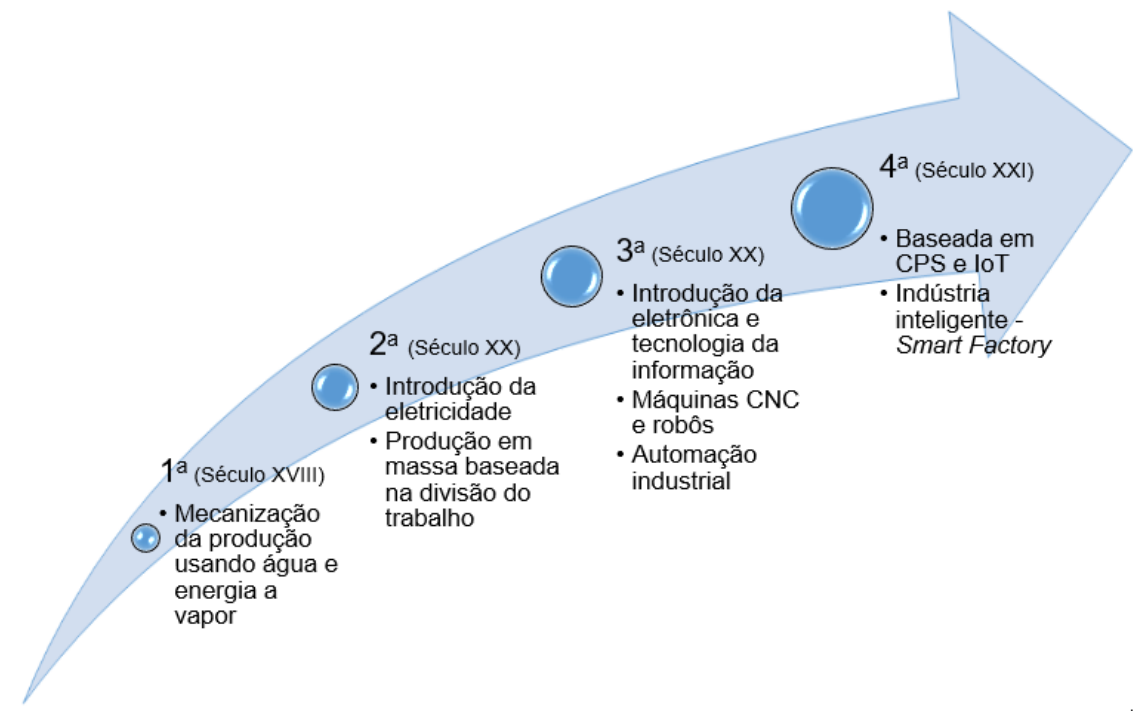
\includegraphics[scale = .4]{Imagens/Introducao/Contextualizacao/evolucoes-industriais.png}
    \centering
    \vspace{0.2cm} \\
    Fonte: \textcite{PISCHING2017}.
    \label{fig:revolucoes_industriais}
\end{figure}

\par Atualmente, vive-se a quarta fase, a chamada Indústria 4.0. Baseada na indústria inteligente, na Internet das Coisas (IoT) e nos sistemas ciber-físicos (CPS - Cyber-Physical Systems), nos quais subsistemas computacionais cooperam entre si e permanecem integrados ao mundo físico e seus processos, permitindo medir, controlar e analisar dados em tempo real por meio da rede, inclusive a Internet \cite{BIGHETI2020,MONOSTORI2016_CPS_MANUFACTURING}.

\par A Figura~\ref{fig:piramide_automacao} resume, em forma de pirâmide, como costuma ser organizada a automação na Indústria 4.0. No nível 0 está o próprio processo físico, no nível 1, sensores e atuadores, por exemplo, um medidor de nível em malha 4-20 mA ou uma válvula de controle. No nível 2 entram os controladores lógicos programáveis (CLPs), que conversam com o nível 1 por protocolos seriais ou, de modo mais direto, pelas entradas e saídas (I/O) do equipamento. Nos níveis 3 e 4 aparecem, respectivamente, os sistemas supervisórios para acompanhar e comandar o processo em tempo real e a camada de gestão empresarial, em que se destacam os ERPs \cite{BIGHETI2020,COLOMBO2014_STATE_ART_AUTOMATION}.

\par Nos últimos anos, os níveis 3 e 4 foram ganhando ainda mais peso: ao digitalizar serviços antes ligados só ao ambiente físico da planta, tornou-se comum ofertá-los também sobre infraestrutura de computação em nuvem e permitir que sejam compartilhados entre diferentes sistemas e usuários. Em linhas gerais, a implementação e o gerenciamento desses serviços seguem a ideia da arquitetura orientada a serviços (Service Oriented Architecture - SOA), materializada por meio de serviços Web (Web Services - WS) \cite{COLOMBO2014_STATE_ART_AUTOMATION}.

\begin{figure}[H]
    \centering
    \caption{Pirâmide de Automação}
    \centering
    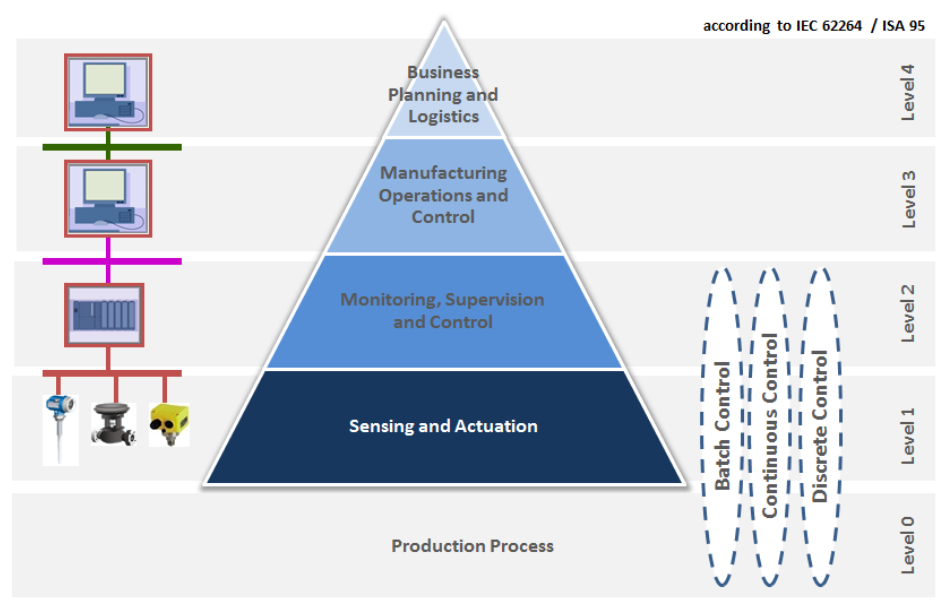
\includegraphics[scale = .5]{Imagens/Introducao/Contextualizacao/piramide-automacao.png}
    \centering
    \vspace{0.2cm} \\
    Fonte: \textcite{COLOMBO2014_STATE_ART_AUTOMATION}.
    \label{fig:piramide_automacao}
\end{figure}

\par A Indústria 4.0 caracteriza-se pelo grande avanço dos protocolos de comunicação e telemetria, aliada à estar no mesmo momento de popularização do desenvolvimento de software e à interconexão de máquinas e sistemas de forma inteligente. Tais avanços permitiram o monitoramento e a supervisão centralizada de processos complexos em tempo real, elevando o papel dos sistemas supervisórios de simples interfaces de operação para centrais estratégicas de análise de dados. Nesse cenário, este trabalho propõe o desenvolvimento de um sistema supervisório web orientado a serviços.